\section{Preliminaries}
\subsection{Problem}
Consider the following discrete-time trajectory optimization problem:
 
\begin{equation}
    \begin{aligned}
        \min_{\boldsymbol{X},\boldsymbol{U}} & \quad J(\boldsymbol{X}, \boldsymbol{U}) = \phi_T(\mathbf{x}_T) + \sum_{k=0}^{N-1} L(\mathbf{x}_k, \mathbf{u}_k) \\
        \text{subject to} & \quad \mathbf{x}_{k} = \boldsymbol{f}(\mathbf{x}_{k-1}, \mathbf{u}_{k-1}), \quad k = 1, 2, \ldots, N
    \end{aligned}
    \label{eq:problem}
\end{equation}
where $\mathbf{x}_k \in \mathbf{R}^n, \mathbf{u}_k \in \mathbf{R}^m$ are the state and control vectors at time step $k$. $\boldsymbol{X} = [\mathbf{x}_1, \mathbf{x}_2, \ldots, \mathbf{x}_N]$ is the state trajectory, $\boldsymbol{U} = [\mathbf{u}_1, \mathbf{u}_2, \ldots, \mathbf{u}_{N-1}]$ is the control trajectory, $\phi_N: \mathbf{R}^n \to \mathbf{R}$ is the terminal cost function, $l: \mathbf{R}^n \times \mathbf{R}^m \to \mathbf{R}$ is the running cost function, and $\boldsymbol{f}: \mathbf{R}^n \times \mathbf{R}^m \to \mathbf{R}^n$ is the system dynamics function.\\
We denote the cost (return) function starting from step $r$ as follows:

\begin{equation}
    J_r = \phi_N(\mathbf{x}_N) + \sum_{k=r}^{N-1} l(\mathbf{x}_k, \mathbf{u}_k)
\end{equation}
The \textbf{value function} is defined as the optimal value of the cost function starting from time step $r$:
\begin{equation}
    V_r(\mathbf{x}_r) = \min_{\boldsymbol{X},\boldsymbol{U}} J_r
\end{equation}
The problem \ref{eq:problem} is now to minimize $J_1$ with respect to control sequence $\boldsymbol{U}$, given the initial state $\mathbf{x}_0$ and the system dynamics.\\
\begin{center}
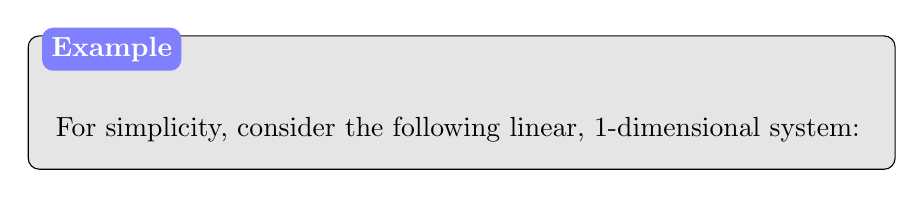
\begin{tikzpicture}
\node[
    draw,
    fill=gray!20,
    rounded corners,
    text width=0.85\textwidth,
    align=left,
    inner sep=10pt
] (box) {
    \vspace{0.5cm}

    For simplicity, consider the following linear, 1-dimensional system:
    % \begin{equation}
    %     x_{k+1} = x_k + u_k
    % \end{equation}
};

\node[
    fill=blue!50,
    text=white,
    rounded corners,
    anchor=west
] at ([xshift=5pt,yshift=-5pt]box.north west)
{\textbf{Example}};
\end{tikzpicture}
\end{center}


\subsection{Second-order method}
A norminal control sequence $\{\mathbf{u}_k, k=1,2,\ldots,N-1\}$ is chosen and the corresponding state trajectory $\{\mathbf{x}_k, k=1,2,\ldots,N\}$ is generated by forward simulating the system dynamics. These sequences are stored. Then we proceed, in reverse time, from $k=N-1$ to $k=1$, to chose an optimal incremental control sequence:

\begin{equation}
    \delta \mathbf{u}_k = \mathbf{g}_k(\delta \mathbf{x}_k)
    \label{eqn: general control law}
\end{equation}
valid for a small region about the initial trajectory and which improve the control and state sequences to be calculated. An incremental $\delta \mathbf{x}_k, \delta \mathbf{u}_k$ will lead to an incremental $\triangle V_k$ and we want to optimize it, e.g:

\begin{equation}
    \begin{aligned}
    \delta \mathbf{u}_k &= \arg \min_{\delta \mathbf{u}_k} \triangle J_k(\delta \mathbf{x}_k, \delta \mathbf{u}_k)\\
    \text{subject to:} & \quad \delta \mathbf{u}_k = \mathbf{g}_k(\delta \mathbf{x}_k)
    \end{aligned}
\end{equation}

Since from \ref{eq:problem}, $\delta \mathbf{x}_{k+r}$ is a function of $\delta \mathbf{x}_k, \delta \mathbf{u}_k, \ldots , \delta \mathbf{u}_{k+r-1}$, then the incremental in the cost function starting from step $k, \triangle V_k$ is a function of $\delta \mathbf{x}_k, \delta \mathbf{u}_k, \ldots , \delta \mathbf{u}_{N-1}$ and if we select the incremental $\delta \mathbf{u}_k$ as in \ref{eqn: general control law}, then the optimal increment $\triangle V_k$ is a function of $\delta \mathbf{x}_k$:
\begin{equation}
    \triangle V_k(\delta \mathbf{x}_k) = \min_{\delta \mathbf{u}_k, \ldots, \delta \mathbf{u}_{N-1}} \triangle J_k(\delta \mathbf{x}_k, \delta \mathbf{u}_k \ldots, \delta \mathbf{u}_{N-1})
\end{equation}
Of course $\triangle V_k(\delta \mathbf{x}_k)$ is a function of $\mathbf{x}_1$ and initial control sequence $\{\mathbf{u}_k, k=1,2,\ldots,N-1\}$. If we assume that $\delta \mathbf{x}_k$ is sufficiently small, then we can approximate $\triangle V^o_k(\delta \mathbf{x}_k)$ by a second-order Taylor expansion:

\begin{equation}
    \triangle V_k(\delta \mathbf{x}_k) = \frac{1}{2} \delta \mathbf{x}_k^T J_{xxk} \delta \mathbf{x}_k + \delta \mathbf{x}_k^T J_{xk} + \mathbf{a}_k
\end{equation}
where we write $ J_{xxk} = \partial^2 J_k/ \partial \mathbf{x}_k ^2$, second derivative of $J_k (\mathbf{x}_k)$ for short. \\
Using the Dynamic Programming principle we have:
\begin{equation}
   \triangle V_k(\delta \mathbf{x}_k) = \min_{\delta \mathbf{u}_k} \left[ \triangle L(\delta \mathbf{x}_k, \delta \mathbf{u}_k) + \triangle V^o_{k+1}(\delta \mathbf{x}_{k+1})\right]
\end{equation}
For simplicity, we consider the case when $\delta \mathbf{x}_k$ and $\delta \mathbf{u}_k$ are scalars, and expand $\triangle L(\delta \mathbf{x}_k, \delta \mathbf{u}_k)$ to the second order Taylor expansion:
\begin{equation}
    \triangle L(\delta \mathbf{x}_k, \delta \mathbf{u}_k) = \frac{1}{2} \begin{bmatrix}
    \delta x_k\\
    \delta u_k
    \end{bmatrix}^T
    \begin{bmatrix}
    L_{xx} & L_{xu}\\
    L_{ux} & L_{uu}
    \end{bmatrix}_k
    \begin{bmatrix}
    \delta x_k\\
    \delta u_k
    \end{bmatrix} + 
    \begin{bmatrix}
    L_{x}\\
    L_{u}
    \end{bmatrix}_k^T
    \begin{bmatrix}
    \delta x_k\\
    \delta u_k
    \end{bmatrix} + a_k
\end{equation}